\documentclass[conference,a4paper]{IEEEtran}
% Shared IEEE-compatible packages. Compiles with pdfLaTeX on Overleaf.
\usepackage[T1]{fontenc}
\usepackage[utf8]{inputenc}
\usepackage{cite}
\usepackage{amsmath,amssymb}
\usepackage{graphicx}
\usepackage{booktabs,array,tabularx}
\usepackage{url}
\usepackage{xcolor}
\usepackage{tikz}
\usepackage{placeins}
\usetikzlibrary{arrows.meta,positioning,shapes.geometric,fit}
\usepackage[breaklinks=true,hidelinks]{hyperref}
\hypersetup{pdfauthor={},pdfsubject={FinPilot AI synthetic sandbox competition documentation}}
\graphicspath{{figures/}}
\newcommand{\project}{FinPilot AI}
\newcommand{\RepoLink}{\url{https://github.com/Shariar-Joy/finpilot-ai}}
\newcommand{\VerifiedCI}{\href{https://github.com/Shariar-Joy/finpilot-ai/actions/runs/39220992552}{verified CI run 39220992552}}
\newcommand{\field}[1]{\rule{#1}{0.35pt}}
\newcommand{\teamAuthors}{\author{%
\IEEEauthorblockN{\field{48mm}}
\IEEEauthorblockA{Team member 1\\Institution: \field{34mm}\\Email: \field{40mm}}
\and
\IEEEauthorblockN{\field{48mm}}
\IEEEauthorblockA{Team member 2\\Institution: \field{34mm}\\Email: \field{40mm}}}}
\newcolumntype{L}[1]{>{\raggedright\arraybackslash}p{#1}}
\definecolor{navy}{HTML}{16233B}
\definecolor{teal}{HTML}{177F78}
\definecolor{lightgray}{HTML}{F2F4F7}
\tikzset{box/.style={draw=navy,rounded corners=2pt,fill=lightgray,align=center,font=\footnotesize,minimum height=11mm,text width=28mm},flow/.style={-{Stealth[length=2mm]},thick,draw=navy},optional/.style={flow,dashed,draw=teal}}
% Generated from actual executed results. Do not change counts by hand.
\newcommand{\UnitTests}{61}
\newcommand{\BrowserTests}{4}
\newcommand{\PythonTests}{8}
\newcommand{\RecordedTransactions}{134}
\newcommand{\AgentMedian}{0.534}
\newcommand{\AgentPninetyfive}{0.827}
\newcommand{\EvidenceDate}{19 October 2026}
\newcommand{\DemoSeconds}{84}


\title{FinPilot AI Sandbox Execution Evidence and Reproduction Guide}
\teamAuthors
\begin{document}
\maketitle
\begin{abstract}
This companion report links the implemented FinPilot AI workflow to reproducible commands, real interface captures, actual synthetic-account audit records, and the recorded limits of verification. It supports the International Track's source-code and non-on-chain execution-evidence requirements. The principal task is a spending explanation followed by a reviewed budget decision. All accounts and amounts are synthetic. Screenshots and logs are evidence of executed application behavior, not invented transactions or generated interface mockups.
\end{abstract}

\section{Artifact and Environment Record}
The source repository is \RepoLink. Technical details are in the main paper; permission tiers and known risks are in the security companion. The repository includes setup instructions, PostgreSQL schema and migration, seed generation, test cases, Python service, real screenshots, sanitized audit JSON, benchmark JSON, and exact local execution logs.

The local verification environment used Windows, Node.js 24.13.0, npm 11.6.2, Python 3.14.2, Next.js 16.4.2, Prisma 6.19.3, and Chromium driven by Playwright. Npm package versions are recorded in the lockfile. The fixed-seed benchmark uses 19 October 2026 at 12:00 UTC and \RecordedTransactions{} transactions over 90 calendar days. The interactive demo instead seeds relative to its actual UTC date; transaction IDs are freshly generated, so their values differ between runs without changing the fixed-seed arithmetic.

\section{Local Reproduction}
\subsection{Keyless Synthetic Demo}
From the checkout, install with \texttt{npm ci}, then run \texttt{npm run dev}. Open \url{http://127.0.0.1:3000}, select ``Explore the live demo,'' and inspect the storage label. The button creates a fresh isolated synthetic workspace; there is no shared password. In-memory mode is sufficient for the entire guided task but loses all data when that process stops.

For persistence, configure DATABASE\_URL, a 32-character-or-longer SESSION\_SECRET, APP\_ORIGIN, and a chosen DEMO\_PASSWORD. Start PostgreSQL, run \texttt{npm run db:migrate}, then \texttt{npm run seed}. The named demo account is created only after the seed command succeeds. An unreachable configured database does not become a memory demo automatically.

The optional private Python service uses the pinned requirements and an ANALYTICS\_SERVICE\_TOKEN shared only with Next.js. Its verified role is independent monthly arithmetic, not permission or budget mutation. The model key is optional; no key is needed for the guided scenario. All credentials are environment variables rather than repository content.

\subsection{Golden Scenario}
In ``AI copilot,'' select ``Run demo scenario.'' The application asks why dining spending increased this month and proposes a next-month limit 20\% lower. Expand the real summary, comparison, transaction-list, budget-status and proposal tool results. Inspect the same-period totals, counts, mean amounts, and transaction evidence. The fixed-seed run reports USD~648.10 versus USD~241.50 and proposes USD~518.48 for November.

Choose ``Reject'' first. Confirm that the existing next-month budget remains unchanged and the audit decision is rejected. Run a fresh scenario and choose ``Approve change.'' Select next month in Budgets and confirm the exact dining limit, then inspect the approved mutation and correlation ID in Activity. A proposal, a decision, and a committed change are separate visible stages.

\begin{figure*}[t]
\centering
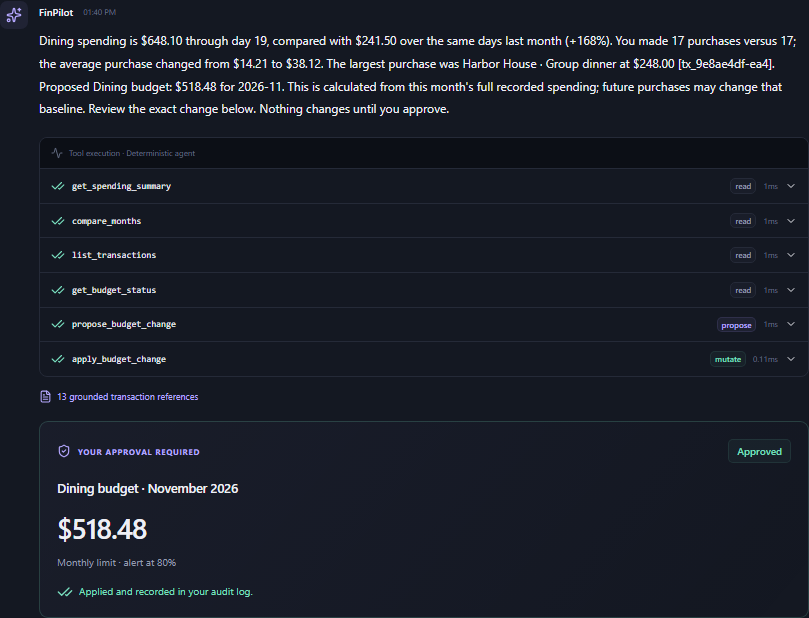
\includegraphics[width=.98\textwidth]{agent.png}
\caption{Actual approved synthetic budget workflow. The tool timeline and transaction references accompany the exact reviewed limit. The screenshot records the running UI; the complete underlying sanitized decision events are supplied separately as JSON.}
\label{fig:agent}
\end{figure*}

\section{Execution Evidence}
\subsection{Recorded Decisions}
Each audit event records the actor, decision, action, UTC timestamp, correlation ID, and explicit metadata. Proposal and decision entries share a proposal identifier and payload hash; different HTTP requests can have distinct correlation IDs. The accompanying JSON contains actual proposed, approved, and rejected events captured through the interface. It excludes session/approval tokens, passwords, API keys, and raw financial text.

The repository also includes browser assertions that compare the complete budget array before and after rejection, check that approval writes the proposed exact limit, and verify audit visibility. Source-level tests reject payload tampering, cross-user attempts, expiration and replay, and require exactly one success under concurrent reuse of a token.

\subsection{Executed Commands}
\begin{table}[t]
\caption{Local command outcomes; full output is retained}
\centering\small
\begin{tabular}{L{43mm}L{35mm}}
\toprule Command & Recorded result\\\midrule
\texttt{npm run lint} & Pass\\
\texttt{npm run typecheck} & Pass\\
\texttt{npm run test} & \UnitTests{} checks passed\\
\texttt{npm run test:e2e} & \BrowserTests{} scenarios passed\\
\texttt{python -m unittest ...} & \PythonTests{} checks passed\\
\texttt{npm run seed} & Synthetic seed verified\\
\texttt{npm run build} & Production build passed\\
\texttt{verify-services.mjs} & Production/Python totals agree\\
\texttt{benchmark.ts} & Fixed-seed data and timings saved\\
\bottomrule
\end{tabular}
\end{table}

The four browser scenarios cover the approval/rejection task, CSV validation and category editing, budget CRUD and reminder approval/completion, and mobile navigation/theme/dialog operation. Domain/API checks cover arithmetic, dates, analysis rules, imports, ownership, sessions, approval security, repository atomicity and provider boundaries. Python checks validate schema, token enforcement, integer totals and body bounds. The refreshed review report enumerates corrected defects and the final executed counts.

\subsection{Microbenchmark}
The benchmark executes ten warm-up and 100 measured deterministic agent runs with a new ledger copy per run. Seed construction is outside the timer. Median time is \AgentMedian{}~ms and the 95th percentile is \AgentPninetyfive{}~ms locally. This measurement excludes HTTP, rendering, storage, and external models. It must not be described as browser response latency or compared with model-service throughput.

\section{Five-Minute Recording Plan}
\begin{enumerate}
\item 0:00--0:30: identify Topic A, the synthetic sandbox, and the problem of turning an explanation into a controlled action.
\item 0:30--1:15: show real ledger-derived cards and charts, transaction search, and source IDs.
\item 1:15--2:00: import a CSV, show validation, duplicate detection, and explicit commit. Demonstrate an invalid date rejecting the batch if time permits.
\item 2:00--3:40: run the dining scenario, inspect tools/evidence, review the exact limit, approve, and show next month's budget and audit record.
\item 3:40--4:20: repeat and reject; verify unchanged financial state and a recorded rejection.
\item 4:20--5:00: summarize the read/propose/apply boundary, known limits, and reproducible source.
\end{enumerate}
The package includes an actual \DemoSeconds{}-second captioned WebM recording, generated by executing the application workflow in Chromium. It has no audio narration; the captions describe observed actions without changing financial results. The recording verifies approval, a separate rejection with unchanged budgets, CSV preview and the audit trail. Recording metadata and the reproduction script accompany the video. The supplied appendix describes a demo video as optional in one checklist item while also mentioning a video under non-on-chain execution evidence~\cite{competition}; the supplied clip is below the five-minute limit. A longer optional recording plan is included above. No presentation deck is included, as requested; a separate Gamma prompt is provided.

\section{Limits of the Evidence}
The local environment had no running PostgreSQL instance. The subsequent \VerifiedCI{} used a real PostgreSQL 17 service: migration and all 61 domain/API cases passed. Its application job passed clean installation, lint, types, 61 memory cases, 8 Python cases, production build, and 4 Chromium scenarios. The repository retains the run URL, exact commit, and observed job/step outcomes in \texttt{ci-verification.json}; repeated storage-adapter runs do not increase the unique test count. Target deployment and restart recovery remain unverified. Provider calls were mocked and the keyless path was exercised; no live paid model call occurred. Docker images were not built locally. There is no public application deployment, user study, load test, external notification, bank integration, transfer, or independent security certification.

The captured UI and benchmark use synthetic data only. Tests establish the behavior of their asserted cases; they do not prove complete security or general financial reasoning accuracy. The team should replace identity fields, review every claim, and attach the actual source URL and required recording before submission.

\FloatBarrier
\bibliographystyle{IEEEtran}
\bibliography{references}
\end{document}
